\documentclass[a4paper,12pt]{article}
\usepackage[utf8]{inputenc}
\usepackage[dutch]{babel}
\usepackage{geometry}
\usepackage{graphicx}
\usepackage{amsmath, amssymb}
\usepackage{setspace}
\usepackage{tocbibind} % Zorgt ervoor dat de inhoudsopgave en voorwoord in de inhoudsopgave verschijnen
\usepackage{array} % Voor betere tabelopmaak
\usepackage{tocloft}
\usepackage{multicol}
\usepackage{tikz}
\usetikzlibrary{arrows.meta, positioning}
\usepackage[hidelinks]{hyperref}

% lente raam 1,96

% Define custom section numbering
\renewcommand{\thesection}{\Alph{section}}
\renewcommand{\thesubsection}{\thesection.\arabic{subsection}}

% Define section and subsection format in Table of Contents
\renewcommand{\cftsecaftersnum}{.}
\renewcommand{\cftsubsecaftersnum}{.}
\renewcommand{\baselinestretch}{1.15}

\setlength{\parskip}{0.8em}
\setlength{\parindent}{0pt}

\geometry{a4paper, top=3cm, bottom=3cm, left=3cm, right=3cm}

\begin{document}

\begin{titlepage}

    \centering
    \vspace*{2cm}

    \Huge
    \textbf{Reinforcement Learning en Computerspellen}

    \vspace{1.5cm}

    
\includegraphics[width=0.175\textwidth]{logo-clz.png} % Voeg breedte toe voor schaal

    \vspace{1.5cm}

    \large
    \textbf{Matthijs Gorter} \\
    \textbf{Thom Brinkhorst} \\
    \textbf{Pepijn van Iperen} \\

    \vspace{1.5cm}

    \large
    Profielwerkstuk \\
    onder begeleiding van \\
    \textbf{S. Rook} \\
    Christelijk Lyceum Zeist \\
    Natuur en Techniek \\
    Februari 2025 \\

    \vfill

\end{titlepage}
% Voorwoord
\newpage
\section*{Voorwoord}
\addcontentsline{toc}{section}{Voorwoord} % Voeg toe aan de inhoudsopgave
Voorwoord inhoud hier. Bedank mensen die geholpen hebben, beschrijf het doel van het profielwerkstuk en eventuele persoonlijke motieven of ervaringen.

\vspace{1cm}
\noindent
Matthijs Gorter, Thom Brinkhorst, Pepijn van Iperen \\
Christelijk Lyceum Zeist \\
Februari 2025

% Variabelen en Notatie
\newpage
\section*{Variabelen en Notatie}
\addcontentsline{toc}{section}{Variabelen en Notatie} % Voeg toe aan de Inhoudsopgave


\begin{table}[h]
    \centering
    \begin{tabular}{>{\raggedright}p{3cm} >{\raggedright\arraybackslash}p{10cm}}
        \textbf{Variabele/ functie} & \textbf{Definitie}                                \\
        \hline
        $t$                         & Tijdstap                                          \\
        $T$                         & Laatste tijdstap van een episode (horizon)        \\
        $x$                         & Toestand (state)                                  \\
        $x_t$                       & Toestand op tijdstip $t$                          \\
        $x'$                        & Toestand een tijdstap na $x$                      \\
        $\mathcal{X}$               & Set van alle toestanden                           \\
        $a$                         & Actie                                             \\
        $\mathcal{A}$               & Alle mogelijke acties                             \\
        $a_t$                       & Actie op tijdstip $t$                             \\
        $r$                         & Beloning (reward)                                 \\
        $\mathcal{R}$               & Set van mogelijke beloningen                      \\
        $r_t$                       & Beloning op tijdstip $t$                          \\
        $r(x, a)$                   & Beloningsfunctie                                  \\
        $\mu$                       & Deterministisch beleid                            \\
        $\pi$                       & Stochastisch beleid                               \\
        $\pi^*$                     & Optimale stochastisch beleid                      \\
        $\gamma$                    & Kortingsfactor tussen 0 en 1                      \\
        $p(x'|x, a)$                & Overgangswaarschijnlijkheidsfunctie               \\
        $\mathcal{P}$               & Overgangswaarschijnlijkheidsmatrix                \\
        $V(x)$                      & Waardefunctie                                     \\
        $Q(x, a)$                   & Q-functie                                         \\
        $Q^*(x, a)$                 & Q-functie met het optimale beleid                 \\
        $\mathbb{E}[X]$             & Verwachtingswaarde van variabele $X$              \\
        $\mathbb{E}[a|b]$           & Geconditioneerde verwachtingswaarde               \\
        $\mathbb{E}_{\pi}[X]$       & Verwachtingswaarde als beleid $\pi$ wordt gevolgd \\
    \end{tabular}
    \caption{Variabelen en Notatie}
\end{table}

% Inhoudsopgave
\newpage
\tableofcontents

% Hoofdstukken
\newpage
\section{Inleiding}
Introductie Onderwerp \\ Onderwerpkeuze verantwoorden \\
Onderzoeksvraag/Hoofdvraag met eventuele hypothese \\ Deelvragen \\ Wat zijn de
specifieke kenmerken van verschillende soorten computerspellen? \\ Welke
reinforcement learning-algoritmes zijn beschikbaar en wat zijn hun kenmerken?
\\ Hoe beïnvloeden de spelkenmerken de prestatie van reinforcement
learning-algoritmes? \\ klein stukje theorie als inleiding op het
theorie-onderdeel \\ werkplan in grote lijnen, opbouw van verslag \\

\newpage
\section{Theoretisch Kader}
\subsection{Definitie}
Reinforcement Learning (RL) is een tak binnen kunstmatige intelligentie waarin
een agent leert door interactie met zijn omgeving. Een agent is een entiteit
die leert en acties onderneemt. Bij een zelfrijdende auto is het
besturingssysteem de agent, en bij een schaakspel is de schaker de agent. De
omgeving is alles waarmee de agent interageert en die reageert op de acties van
de agent. Bij een zelfrijdende auto is dit de weg waar de auto op rijdt en de
voertuigen om de auto heen. Bij een schaakspel is dit het schaakbord.

De agent leert door interactie met zijn omgeving. De agent ontvangt beloningen
of straffen (negatieve beloningen) als gevolg van zijn acties. Het doel van de
agent is om een strategie te ontwikkelen die de cumulatieve beloning
maximaliseert over tijd. Bij Super Mario Bros (1985) is Mario de agent en de
agent krijgt een beloning als Mario richting de eindslag beweegt (meestal naar
rechts) en als Mario een coin of een power up oppakt en Mario krijgt een straf
als Mario sterft en hij krijgt elke seconde straf zodat hij zo snel mogelijk
het level wilt voltooien.

\begin{figure}[h]
    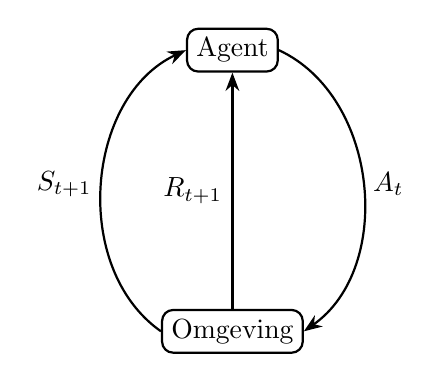
\begin{tikzpicture}[auto, thick, node distance=2cm,>=Stealth]
        \node[draw, rectangle, rounded corners] (agent) {Agent};
        \node[draw, rectangle, rounded corners, below=of agent, yshift=-1cm] (environment) {Omgeving};

        % Action arrow with adjusted bend
        \draw[->] (agent.east) to[bend left=60] node[midway, right] {$A_t$} (environment.east);

        % State arrow with adjusted text position
        \draw[->] (environment.north) tonode[midway, left] {$R_{t+1}$} (agent.south);

        % Reward arrow with adjusted text position
        \draw[->] (environment.west) to[bend left=60] node[midway, left] {$S_{t+1}$} (agent.west);
    \end{tikzpicture}
    \caption{Reinforcement learning interactiemodel tussen agent en omgeving via acties, toestanden en beloningen.}
\end{figure}

Een actie naar de beslissing die een agent neemt bij elke
stap in een besluitvormingsproces. Acties worden aangeduid met \( a \) en
worden gekozen uit een reeks mogelijke acties \( \mathcal{A} \). Elke door de
agent genomen actie beïnvloedt de interactie met de omgeving, wat leidt tot een
verandering in de toestand en een daaruit voortvloeiende beloning.

\subsection{Belangrijke Reinforcement Learning-Algoritmes}
\subsection{Vergelijking met andere Artificiële Leermethodes}
\subsection{Reinforcement Learning in Computerspellen}

\newpage
\section{Onderzoeksmethoden}
\newpage
\section{Analyse en Resultaten}
\newpage
\section{Conclusie}
\newpage
\section{Discussie}
\newpage
\section{Bronvermelding}
\newpage
\section{Bijlagen}

% Meer secties of hoofdstukken kunnen hier toegevoegd worden

\end{document}